%% HeatGraph manuscript -- Elsevier elsarticle, author-year citations.
%% Compile: tectonic main.tex (or pdflatex + bibtex, or Overleaf).
%% Numbers in this file are taken from manuscript/facts.json (built from the saved results) and are
%% audited by manuscript/check_numbers.py. Figures and tables are byte-identical copies of ../figures, ../tables.
\documentclass[preprint,12pt,authoryear]{elsarticle}

\usepackage{iftex}
\ifPDFTeX                      % pdflatex (e.g. Overleaf default)
  \usepackage[T1]{fontenc}
  \usepackage[utf8]{inputenc}
  \usepackage{lmodern}
  \DeclareUnicodeCharacter{2010}{-}
\else                          % XeTeX / LuaTeX (e.g. tectonic): Unicode Latin Modern
  \usepackage{fontspec}
\fi
\usepackage{amsmath,amssymb}
\usepackage{graphicx}
\usepackage{booktabs}
\usepackage{makecell}
\setlength{\abovetopsep}{6pt}   % space between a table caption and its top rule
\usepackage{pdflscape}
\usepackage{url}
\usepackage[hidelinks]{hyperref}
\usepackage{xcolor}
\usepackage[a4paper,margin=2.5cm]{geometry}

\hypersetup{pdftitle={Where should street trees go? Exposure-weighted allocation with physics-informed surrogates},
            pdfauthor={Mohammad Baradaran Aghghaleh, Khorshid Mehrabi, Ali Yazdani}}
\pdfstringdefDisableCommands{\def\corref#1{}}
\setlength{\emergencystretch}{1.5em}
\renewcommand{\topfraction}{0.9}
\renewcommand{\bottomfraction}{0.8}
\renewcommand{\textfraction}{0.1}
\renewcommand{\floatpagefraction}{0.75}
\setcounter{topnumber}{3}
\setcounter{totalnumber}{4}

\graphicspath{{figures/}}
\newcommand{\degC}{\ensuremath{^\circ}C}
\newcommand{\tmrt}{\ensuremath{T_\mathrm{mrt}}}

\journal{Landscape and Urban Planning}

% elsarticle's first-page footer leaves a stray space after its \textwidth box (2.6 pt overfull); same footer without it
\makeatletter
\def\ps@pprintTitle{\let\@oddhead\@empty\let\@evenhead\@empty
  \def\@oddfoot{\hbox to \textwidth{\footnotesize\itshape Preprint submitted to \@journal\hfill\@date}}%
  \let\@evenfoot\@oddfoot}
\makeatother

\begin{document}

\begin{frontmatter}

\title{Where should street trees go? Exposure-weighted allocation with physics-informed surrogates, tested against practitioner rules and verified with SOLWEIG}

\author[aff1]{Mohammad Baradaran Aghghaleh}
\author[aff1]{Khorshid Mehrabi}
\author[aff1]{Ali Yazdani\corref{cor1}}
\cortext[cor1]{Corresponding author.}
\affiliation[aff1]{organization={Department of Urban Planning, Science and Research Branch, Islamic Azad University},
            city={Tehran},
            country={Iran}}

\begin{abstract}
Planners must decide where a limited number of street trees will most reduce pedestrian heat stress. We weighted tree cooling by pedestrian flow and compared model-based allocation with random planting and a practitioner rule in four unseen neighbourhoods of two cities. A calibrated 2.5D radiation and Universal Thermal Climate Index (UTCI) engine reproduced SOLWEIG-GPU mean radiant temperature on held-out days with mean absolute errors of 1.30--1.62~K. A graph neural network (GNN) with physics-informed crown-shadow features predicted tree-induced UTCI change in an unseen city with an error of 0.063~\degC. In a German city whose building heights were largely imputed, the error was 0.075~\degC. The two errors were 66\% and 61\% below a no-change reference, and a linear model on the same features came close. Model-based allocation reduced engine-verified pedestrian heat dose 1.8--6.0 times more than random layouts. A practitioner rule that plants the sunniest, busiest streets achieved only 46--85\% of that reduction, and 29--71\% when pedestrian flow was ignored. Greedy allocation matched multi-objective search on cooling; the search added layouts that reduced between-district inequality by up to 8.2\% at 90\% of greedy's cooling, mainly by cooling the least exposed district less. In a cross-model check, SOLWEIG-GPU confirmed the cooling of optimised layouts, with per-segment correlations of 0.91--0.94. Our engine and GNN underestimated it by 10--20\% and 11--21\% in total but concentrated it more under new crowns. Where trees go matters as much as how many are planted, and a transparent greedy allocation on shading features captures most of the attainable cooling.
\end{abstract}

\begin{keyword}
Urban heat \sep Street trees \sep Tree planting strategy \sep Pedestrian heat exposure \sep Thermal comfort \sep Graph neural networks \sep Multi-objective optimisation
\end{keyword}

\end{frontmatter}

%% ==========================================================================================
\section{Introduction}\label{sec:intro}

Daytime outdoor heat stress in streets is governed less by air temperature than by radiation~\citep{thorsson2007,lindberg2008}. In sunlit canyons the mean radiant temperature (\tmrt) can exceed air temperature by tens of kelvin, and shade is the most direct way to lower it~\citep{middel2021}. Street trees provide that shade where people walk. Evidence that urban greening and tree canopy reduce surface and pedestrian heat is consistent across climates and methods~\citep{bowler2010,rahman2020,schwaab2021,lee2016}. The planning question is therefore rarely \emph{whether} to plant, but \emph{where} a constrained number of trees should go.

The answer depends strongly on context. A tree on an unshaded street gives roughly 1.5--2 times the pedestrian radiative cooling of the same tree on a street that is already shaded~\citep{lachapelle2023}. Tree location and arrangement also change microclimate and comfort beyond what canopy fraction alone captures~\citep{zhao2018,ziter2019}.

Answering the \emph{where} question requires evaluating many candidate layouts. Physically based models such as SOLWEIG resolve shadows, sky view and six-directional radiant fluxes at metre resolution~\citep{lindberg2008,lindberg2011,lindberg2018}. Even their GPU implementation~\citep{kamath2026} remains too expensive for the thousands of layouts that a search over hundreds of planting slots requires. Neural surrogates have therefore been trained to emulate SOLWEIG~\citep{briegel2023,briegel2024}, and a neural \tmrt{} approximation has been used to optimise tree placements over large areas~\citep{schrodi2023}. Graph neural networks (GNNs) now also predict street-level temperature and microclimate~\citep{yu2024,xin2025}.

Two limitations recur across this work. First, surrogates are validated on held-out \emph{observed} scenes. An optimiser, however, evaluates thousands of \emph{edited} scenes that differ systematically from the training data, and errors on those edits determine decision quality. Second, the objective is usually heat averaged over space. The people who experience heat walk along a network whose segments carry very different pedestrian flows~\citep{sevtsuk2021,kuras2017}. Heat-aware routing studies model this exposure but take urban form as fixed~\citep{kolaxidis2025,vu2025}. The literature on unequal distribution of canopy and heat~\citep{schwarz2015,hsu2021,mcdonald2021,locke2021,benz2021} rarely enters the allocation algorithm itself. Third, model-based allocations are seldom compared with the simple rules that planners already use, such as planting the sunniest or the busiest streets. Without that comparison it is unclear whether a model is worth its cost.

This paper asks where a fixed number of street trees should go to reduce the heat that pedestrians actually experience, and how much is lost by simpler rules. Its contributions are:
\begin{enumerate}
  \item A planning comparison in four neighbourhoods that the models had not seen, with every outcome re-simulated by a physics engine. Exposure-weighted allocation is compared with random planting and with a practitioner rule that plants the sunniest, busiest streets, which shows how much of the attainable cooling each approach captures.
  \item Evidence that the shading mechanism, encoded as crown-shadow features of each candidate tree, is what transfers to unseen cities. A transparent greedy allocation on these features reaches the cooling optimum that a multi-objective search also finds. The search adds explicit trade-offs between cooling, equity and budget rather than extra cooling.
  \item A fast 2.5D radiation and Universal Thermal Climate Index (UTCI) engine, accepted against SOLWEIG-GPU on held-out patch-days before any learning, and a graph neural network (GNN) surrogate tested on the change that tree planting causes in unseen cities. The GNN improves on a linear model on the same features mainly where crowns overlap.
  \item Cross-model verification of optimised layouts in an unseen city with the full SOLWEIG-GPU model, which was developed independently of our engine.
\end{enumerate}
We also report qualifying results. Multi-objective optimisation did not outperform greedy allocation on cooling and fell short of it when not seeded with the greedy layouts. A linear model on the physics features came close to the GNN, and the equity results rest on a population proxy.

%% ==========================================================================================
\section{Related work}\label{sec:related}

\paragraph{Pedestrian thermal comfort modelling.}
Street-level \tmrt{} is commonly computed with the six-directional flux scheme of \citet{thorsson2007}. SOLWEIG implements this scheme with building and vegetation shadowing on raster height models~\citep{lindberg2008,lindberg2011} and is distributed within the Urban Multi-scale Environmental Predictor (UMEP)~\citep{lindberg2018}. Raster shadow casting makes such models tractable at city scale~\citep{ratti2004}. Crown transmissivity values come from field measurement~\citep{konarska2014}, and the operational UTCI procedure~\citep{brode2012} has an open implementation~\citep{tartarini2020}. Field studies show that shade type and quality strongly modulate comfort~\citep{middel2016,middel2021}. A recently released GPU implementation of SOLWEIG~\citep{kamath2026} provides an independent, scriptable reference for lighter engines, which is how we use it.

\paragraph{Neural surrogates of urban microclimate.}
A U-Net trained on SOLWEIG output reproduced \tmrt{} in Freiburg with a mean absolute error (MAE) of 2.4~K at about 22 times the speed of the physical model~\citep{briegel2023}. It was then embedded in a city-scale thermal-comfort emulator~\citep{briegel2024}. Graph neural networks estimate street-level air temperature~\citep{yu2024}, and UrbanGraph encodes shading and convection in a dynamic heterogeneous graph~\citep{xin2025}. These models build on message passing~\citep{gilmer2017}, inductive neighbourhood aggregation~\citep{hamilton2017}, graph attention~\citep{brody2022} and graph-based physical simulators~\citep{pfaff2021}. Across this literature, accuracy is reported on held-out observed scenes. The accuracy of the \emph{change} caused by an intervention, which is what an optimiser exploits, is rarely measured.

\paragraph{Optimising tree placement.}
Surrogate-assisted search has been used to place trees for minimal \tmrt{}~\citep{schrodi2023}. It has also allocated cool and green roofs by Pareto optimisation under future climate~\citep{kim2025}. These studies minimise heat over space. Because the pedestrian benefit of a tree depends strongly on existing shade~\citep{lachapelle2023}, objectives should instead be defined where people are. Greedy algorithms are provably near-optimal for monotone submodular coverage objectives~\citep{nemhauser1978}. Greedy is therefore a demanding baseline whenever shading is close to additive.

\paragraph{Pedestrian exposure and heat equity.}
Personal heat exposure can differ substantially from area-averaged estimates~\citep{kuras2017}. Pedestrian flows on every street segment can be estimated from network structure and destination attractiveness~\citep{sevtsuk2021}, and street networks are openly available~\citep{boeing2017,osm2026}. Shade-aware routing reduced solar exposure by about 12--26\% in most tested cases~\citep{kolaxidis2025}. Street-view-derived heat has also been mapped onto pedestrian networks with an environmental-justice framing~\citep{vu2025}. Canopy follows income~\citep{schwarz2015}. In urbanised areas of the United States (US), low-income blocks have about 15\% less tree cover and are about 1.5~\degC{} hotter than high-income blocks~\citep{mcdonald2021}. Heat-island exposure is higher for lower-income residents and people of colour in most large US cities~\citep{hsu2021,chakraborty2019,benz2021}, and present canopy tracks historical redlining~\citep{locke2021}. Post-hoc equity analysis of mitigation infrastructure exists~\citep{sanchez2019}, but equity rarely enters the optimiser.

%% ==========================================================================================
\section{Data and methods}\label{sec:methods}

\subsection{Study design and data}\label{sec:data}

We analysed 18 patches (Table~\ref{tab:T1_patches}). Seventeen lie in nine Dutch cities (Almere, Amersfoort, Amsterdam, Delft, Den Haag, Eindhoven, Groningen, Rotterdam, Utrecht), and one lies in Freiburg, Germany. Each patch is a 900~m $\times$ 900~m window at 1~m resolution. It contains a 500~m analysed core and a 200~m buffer that represents shadows and horizons from outside the core. Patches were stratified by intended Local Climate Zone (LCZ)~\citep{stewart2012,demuzere2022}.

Three patches did not initially match their intended typology: a waterfront patch that was mostly river, an office district that was mostly woodland, and a high-rise district. We re-centred them by a reproducible search over 50~m candidate offsets. The search scored core building surface fraction (BSF), area-weighted building height, the number of buildings taller than 40~m and water fraction. The raw dataset was then frozen with a SHA-256 hash for each of its 577 files, and all later steps verify those hashes.

Dutch building footprints and heights come from 3DBAG~\citep{peters2022}, using the 70th-percentile roof height above ground. For Freiburg we used Overture Maps building heights~\citep{overture2026}. Because 65.8\% of these heights were missing, they were imputed from the median of known buildings within 50~m. Freiburg therefore tests transfer across a country border and an input regime: building heights come from a different source and are largely imputed rather than derived from lidar as in 3DBAG. Its engine labels are computed on the same imputed heights that the surrogate sees. The test therefore measures robustness to a shift in the distribution of inputs, not the error caused by wrong heights relative to the true city. Canopy height comes from the global 1~m map of \citet{tolan2024}, which reports a mean absolute error of 2.8~m against aerial lidar. Canopy below 2~m was treated as absent.

The walkable network, destinations and water polygons come from the Overture Maps transportation, place and base themes, which derive from OpenStreetMap~\citep{overture2026,osm2026}. Hourly meteorological forcing comes from the ERA5-based Open-Meteo archive~\citep{hersbach2020,openmeteo2026}. It comprises air temperature, relative humidity, 10~m wind, global, direct and diffuse radiation, and pressure. We used three heatwave days: 25 July 2019, 8 August 2020 and 19 July 2022.

\subsection{Radiation and thermal comfort engine}\label{sec:engine}

The engine computes, per pixel and hour, the sunlit fraction, the sky view factor (SVF), \tmrt{} and UTCI. Solar position follows the solar position algorithm of the National Renewable Energy Laboratory (NREL)~\citep{reda2004} as implemented in pvlib~\citep{holmgren2018}. Because the forcing gives radiation as the mean of the preceding hour, the sun is evaluated at the interval midpoint, which is also SOLWEIG's convention. Shadows are cast on the building and canopy height grids by the shifted-maximum raster method~\citep{ratti2004}. A ray passing through a crown between the trunk-zone top and the crown top is attenuated to a transmissivity of 3\% \citep{konarska2014}. The trunk zone covers the lowest 25\% of tree height. The SVF of a horizontal receptor is
\begin{equation}
  \mathrm{SVF} = \frac{1}{n}\sum_{k=1}^{n}\cos^{2} h_k ,
\end{equation}
where $h_k$ is the horizon elevation in azimuth sector $k$, with $n = 36$ and a search radius of 200~m. Horizons are computed separately for buildings and for buildings plus crowns, and transmissive crowns weight the two.

Following \citet{thorsson2007}, the mean radiant flux density absorbed by a standing person and the resulting \tmrt{} are
\begin{equation}
  S_\mathrm{str} = a_k\Big(\sum_{i=1}^{6} F_i K_i + f_p\, I\, s\Big) + a_l \sum_{i=1}^{6} F_i L_i ,\qquad
  \tmrt = \Big(\frac{S_\mathrm{str}}{a_l\,\sigma}\Big)^{1/4} - 273.15 .
\end{equation}
The angular factors are $F_i = 0.06$ for the upward and downward directions and $0.22$ for the four lateral directions. The absorption coefficients are $a_k = 0.70$ and $a_l = 0.97$. $I$ is direct normal irradiance, $s$ the sunlit fraction, $f_p$ the projected-area factor of a standing person, and $K_i$ and $L_i$ the short-wave and long-wave fluxes. Diffuse and direct radiation come from the forcing, decomposed with \citet{erbs1982} where only global radiation is available. Clear-sky emissivity follows \citet{prata1996}. Ground and wall temperatures rise above air temperature in proportion to absorbed radiation through two coefficients. These coefficients and the ground albedo were calibrated (Section~\ref{sec:calib}). UTCI follows the operational procedure~\citep{brode2012,tartarini2020}. Because UTCI expects 10~m wind, street-level ventilation enters as the forcing wind times an urban reduction factor of 0.5. The result is clipped to the validity range of 0.5--17~m~s$^{-1}$.

For label generation, the same equations are evaluated only at pedestrian receptor pixels and batched over plantings on a GPU. Two exact decompositions make this efficient. The horizon over buildings and crowns is the maximum of a building horizon, computed once, and a canopy horizon. Building shadows do not depend on trees, so they are computed once per hour. Unit tests confirm that the receptor engine reproduces the full-grid engine on synthetic scenes. Agreement in segment UTCI is within $2\times10^{-3}$~\degC{} on both CPU and GPU.

\subsection{Calibration against SOLWEIG-GPU}\label{sec:calib}

Before any learning, the engine had to pass an acceptance gate against SOLWEIG-GPU~\citep{kamath2026}. The gate requires a \tmrt{} mean absolute error of at most 3~K and an absolute bias of at most 1~K over all ground pixel-hours of the 500~m core. Both models received identical rasters and an identical meteorological file. Ground warming, wall warming and ground albedo were fitted by grid search on one patch-day only (Amsterdam Grachtengordel, 25 July 2019). The gate was then evaluated on four held-out patch-days in three cities and two morphologies (Table~\ref{tab:T2_engine_vs_solweig}).

\subsection{Counterfactual tree-planting dataset}\label{sec:dataset}

On each patch we derived street segments from the walk network, keeping segments whose midpoint lies in the core. Pedestrian receptors were placed every 5~m along each segment, excluding building pixels. Candidate planting slots were placed 4~m either side of street-like segments every 12~m. A slot was rejected if its crown disc touched a building or water, or if canopy of at least 2~m already stood there. Slots within 8~m of another slot were also rejected, and at most 250 slots were kept per patch. New trees were crowns of 3~m radius and 8~m height.

For each patch we generated 81 plantings. One is the existing canopy without new trees, which serves as the baseline. The other 80 are random plantings with a slot density drawn uniformly between 2\% and 40\%. Each planting was simulated for the 36 hours from 08:00 to 19:00 local time on the three heatwave days. Segment UTCI is the mean over the segment's receptors. The dataset comprises 1,458 plantings, 52,488 (planting, hour) graphs, 4,889 segments and 35,440 receptors, with 144--250 slots per patch. Generation took 27--54~s per patch on an NVIDIA RTX 5070.

\subsection{Graph representation and physics-informed edges}\label{sec:graph}

Each (planting, hour) pair is a heterogeneous graph with two node types. \emph{Segment} nodes carry static morphology: length, orientation, local building height and building-only SVF. They also carry hourly features: building-only sunlit fraction, solar elevation and azimuth, air temperature, humidity, direct and diffuse radiation, and wind. \emph{Slot} nodes carry a planted flag and crown dimensions. Segments sharing an intersection are linked. Each \emph{planted} slot is linked to every segment whose nearest receptor lies within 25~m.

The slot-to-segment edges carry hour-dependent features. These are the distance, the alignment of the slot-to-receptor vector with the shadow direction, and the ray-height ratio $d\tan e/z_c$. Here $d$ is the distance, $e$ the solar elevation and $z_c$ the crown height. We call these three the \emph{geometric} edge features. The \emph{crown-shadow} representation adds two features that describe the shading mechanism directly. Let $\mathbf{u}$ be the unit vector pointing away from the sun and $z_t$ the trunk-zone height. A crown of radius $\rho$ at slot $\mathbf{p}_k$ then casts a ground shadow that we approximate by a stadium of radius $\rho$. Its axis $\mathcal{S}_k(t)$ runs from $\mathbf{p}_k + (z_t/\tan e)\,\mathbf{u}$ to $\mathbf{p}_k + (z_c/\tan e)\,\mathbf{u}$. For slot $k$, segment $e$ with receptor set $R_e$ and hour $t$,
\begin{equation}
  \begin{gathered}
  \phi^\mathrm{shade}_{ke}(t) = \frac{1}{|R_e|}\sum_{r\in R_e} \mathbf{1}\big[\operatorname{dist}(\mathbf{r},\,\mathcal{S}_k(t)) \le \rho\big]\;\mathbf{1}\big[r \text{ not in building shadow at } t\big],\\
  \phi^\mathrm{over}_{ke} = \frac{1}{|R_e|}\sum_{r\in R_e} \mathbf{1}\big[\lVert \mathbf{r}-\mathbf{p}_k\rVert \le \rho\big].
  \end{gathered}
\end{equation}
$\phi^\mathrm{shade}$ is the share of a segment's receptors that a crown can newly shade at that hour. $\phi^\mathrm{over}$ is the share directly under the crown, a proxy for the reduction in sky view.

\subsection{Surrogate models}\label{sec:surrogates}

The surrogate predicts the tree-induced change in segment UTCI on top of the engine's baseline for the existing canopy, $\hat U_{e,t} = U^\mathrm{base}_{e,t} + f_\theta(\cdot)_{e,t}$. It therefore learns only what trees add. After type-specific encoders, each of three layers updates the segment embeddings $\mathbf{h}_e$ as
\begin{equation}
  \mathbf{h}_e \leftarrow \operatorname{LN}\Big(\mathbf{h}_e + \operatorname{ReLU}\big(\textstyle\sum_{k\in\mathcal{N}_\mathrm{slot}(e)} \operatorname{MLP}([\mathbf{h}_k, \mathbf{a}_{ke}, \mathbf{h}_e]) + \operatorname{SAGE}(\mathbf{h}_e, \{\mathbf{h}_{e'}\}_{e'\in\mathcal{N}_\mathrm{seg}(e)})\big)\Big).
\end{equation}
Here $\mathbf{a}_{ke}$ are the edge features, SAGE is neighbourhood aggregation over adjacent segments~\citep{hamilton2017}, and LN is layer normalisation. Slot messages are \emph{summed} because tree effects are close to additive in the number of crowns.

We compared this model with two alternatives. In an ablation, the slot relation used GATv2 attention~\citep{brody2022}, whose softmax normalisation averages over incoming slots. As a non-graph baseline, we fitted a linear model per hour $t$ of the segment change on $\sum_k \phi^\mathrm{shade}_{ke}(t)$, $\sum_k \phi^\mathrm{over}_{ke}$ and the number of planted links. Models were implemented in PyTorch Geometric~\citep{fey2019} and trained on the GPU. They used 96 hidden units, dropout 0.1 and AdamW~\citep{loshchilov2019} with learning rate $2\times10^{-3}$, weight decay $10^{-4}$, a cosine schedule and batch size 32.

The split was fixed before training. Training used 11 Dutch patches. Model selection and early stopping, with a patience of 10 epochs, used three whole patches from the training cities: Amsterdam Bos en Lommer, Eindhoven Strijp-S and Amersfoort Vathorst. We call this leave-patch-out validation. Evaluation used the three Rotterdam patches, an unseen city, and Freiburg, an unseen city in another country with a different input regime. Neither test set informed any modelling choice. Besides the UTCI error, we report the error and correlation of the predicted \emph{change} against the engine. We also report its skill relative to a no-change reference, which predicts that trees change nothing.

\subsection{Uncertainty quantification}\label{sec:conformal}

Prediction intervals use split conformal prediction~\citep{lei2018,angelopoulos2021}. Intervals are calibrated separately for each of the 36 hours (Mondrian calibration) on the validation patches, on which no model was trained. For calibration residuals $r_i = |y_i - \hat y_i|$ of hour group $h$, the half-width $q_h$ is the $\lceil (n_h+1)(1-\alpha)\rceil$-th smallest residual. This gives marginal coverage of at least $1-\alpha$ for exchangeable data, and we use $\alpha = 0.1$. The optimiser minimises the upper bound $\hat U + q_h$. Because $q_h$ is the same for every segment and every layout at a given hour, it does not penalise layouts whose predictions are more uncertain. Its effect is to lower the heat-stress threshold at hour $h$ from 26~\degC{} to $26 - q_h$, so that segment-hours whose predicted UTCI lies just below the threshold still count. We therefore treat $q_h$ as an hourly threshold-calibration margin rather than as a layout-specific robustness term. We report its empirical coverage on the test patches, both on all counterfactual plantings and on the layouts that the optimiser returned (Section~\ref{sec:res-surrogate}).

\subsection{Exposure, equity and optimisation objectives}\label{sec:objectives}

Pedestrian flows $f_e$ on each segment of the full 900~m network follow a gravity model in the spirit of \citet{sevtsuk2021}. Every node generates the same number of trips. Trips are distributed to destinations, Overture places snapped to the nearest node, in proportion to their count times $\exp(-\beta d)$. We used $\beta = 0.002$~m$^{-1}$ within an 800~m radius and assigned trips to shortest paths. The person-weighted heat dose of a planting $x$ is
\begin{equation}
  D(x) = \sum_{t}\sum_{e} f_e\,\frac{L_e}{v}\,\max\big(\hat U_{e,t}(x) + q_t - 26\,^\circ\mathrm{C},\,0\big),
\end{equation}
with segment length $L_e$ and walking speed $v = 1.3$~m~s$^{-1}$. The threshold of 26~\degC{} is the lower bound of the UTCI \emph{moderate heat stress} category~\citep{brode2012}.

For equity, the 500~m core is divided into four districts, the quadrants obtained by splitting it at its centre along the grid axes. Each segment belongs to the quadrant that contains the centroid of its receptors. The districts are therefore geometric units of equal area, not administrative neighbourhoods. Per-capita dose $x_g$, the dose accumulated on a district's segments divided by its population, is compared across them. We use the population-weighted Theil index $T = \frac{1}{W}\sum_g w_g \frac{x_g}{\mu}\ln\frac{x_g}{\mu}$ \citep{shorrocks1980}. No census data were ingested, so district population $w_g$ is approximated by building floor area. Floor area is the footprint area times the number of storeys implied by the 3DBAG height. Vulnerability weights are set to one. Section~\ref{sec:limitations} discusses this proxy.

\subsection{Optimisation and baselines}\label{sec:optim}

NSGA-III~\citep{deb2014} minimised three objectives: dose, Theil index and number of trees. Budgets were capped at 100 trees, or 40\% of slots. We used pymoo~\citep{blank2020} with two-point crossover, bit-flip mutation and 28 reference directions. The initial population contains the greedy path, that is, the best layout with 1, 2, \ldots{} trees. It also contains swap mutants of each greedy layout, the empty layout and random feasible layouts. Every evaluated layout is kept in an archive, and the returned front is the non-dominated feasible subset of that archive. By construction, the front therefore weakly dominates the greedy layouts used as seeds.

We compared four methods on the three Rotterdam patches and Freiburg at budgets of 5, 10, 20, 30 and 40\% of slots:
\begin{itemize}
  \item NSGA-III on the GNN, the primary method, with 100 individuals and 150 generations;
  \item NSGA-III on the linear surrogate, with 300 generations;
  \item greedy allocation on the linear surrogate, which adds at each step the slot that most reduces the dose bound;
  \item two practitioner heuristics that use no surrogate and no optimiser;
  \item ten random layouts per budget.
\end{itemize}
The heuristics mimic a planner who plants the streets that are sunny and lack canopy. Each street segment receives the score $s_e = f_e\,\bar{\sigma}_e\,(1-c_e)$, where $\bar{\sigma}_e$ is the building-only sunlit share of its receptors averaged over the 36 hours and $c_e$ the share of its receptors under existing canopy of at least 2~m. The \emph{sun-only} variant drops the flow $f_e$. Each candidate slot takes the score of its nearest segment. Trees are then placed one at a time on the slot that maximises $s_e/(1+n_e)$, where $n_e$ is the number of trees already placed on that segment, so that planting spreads along the priority streets.

Because the NSGA-III population is seeded with the greedy layouts, its match with greedy is partly built in. We therefore also ran NSGA-III on the GNN without greedy seeding, with the same population, generations, operators and random seed. Its initial population was the empty layout and random feasible layouts with a uniformly drawn number of trees. We compared the two fronts by their hypervolume in the engine-verified objective space, with dose normalised by the dose without new trees and the number of trees by the number of slots.

For NSGA-III, the layout reported at a budget is the archive layout with the lowest surrogate dose within that budget. Every reported layout was re-simulated with the calibrated engine. All outcomes in Section~\ref{sec:res-bench} are therefore engine values, not surrogate predictions. To see how the equity layouts change the distribution of cooling, we also report the per-district reduction of per-capita dose for greedy and for the equity-selected layout.

\subsection{Sensitivity and stability analyses}\label{sec:sensitivity}

We tested how the allocation results depend on fixed modelling choices, using the engine and the surrogates but no further SOLWEIG runs. Three physical parameters were varied: crown transmissivity (0.01 and 0.10 instead of 0.03), the crown of new trees (a young tree of 2~m radius and 6~m height, and a mature tree of 4~m radius and 12~m height, instead of 3~m and 8~m) and the street wind factor (0.3 and 0.7 instead of 0.5). For each, the greedy, practitioner-heuristic and random layouts of Section~\ref{sec:optim} were re-simulated with the perturbed engine. Two objective parameters were varied: the gravity decay $\beta$ (0.001 and 0.004~m$^{-1}$) and the heat-stress threshold (24 and 28~\degC). Because these change only the objective, greedy was re-run on the linear surrogate under each setting. We then report the engine-verified dose reduction and the overlap of the re-optimised layout with the original greedy layout, measured by the Jaccard index of planted slots. To check that the NSGA-III results do not depend on one random seed, we repeated the NSGA-III (GNN) run with five seeds. For each seed we re-simulated the layout picked at each budget and, from a subsample of 100 front layouts, the equity-selected layout.

\subsection{Cross-model verification with SOLWEIG-GPU}\label{sec:verify}

On Rotterdam Centrum, an unseen city for the surrogate, we took five layouts from the NSGA-III (GNN) front. To avoid selecting on the outcome, we chose them with the GNN's own objectives. They are no new trees, a low budget of about 10\% of slots, the knee of the front, a high budget of about 30\% and maximum cooling. Each layout was simulated with SOLWEIG-GPU for the three heatwave days, giving 15 runs. SOLWEIG UTCI was sampled at the same receptors and averaged per segment for 08:00--19:00. SOLWEIG treats wind differently from our engine. All comparisons therefore use changes relative to each model's own no-planting run. We call a segment-hour \emph{affected} by a layout when a model's UTCI change there is below $-0.05$~\degC, that is, when the layout cools it by more than 0.05~\degC. To compare cooling magnitudes, we average each model's change over the segment-hours that SOLWEIG marks as affected, a mask common to the three models.

%% ==========================================================================================
\section{Results}\label{sec:results}

\subsection{The engine passes the SOLWEIG-GPU acceptance gate}\label{sec:res-engine}

With default parameters the engine ran too cool, and three of the four held-out patch-days failed the bias criterion (Table~\ref{tab:T2_engine_vs_solweig}, Fig.~\ref{fig:F1}). Calibration on the fitting patch-day reduced its mean absolute error from 1.81 to 1.32~K and its bias from $-1.36$ to $-0.40$~K. The fitted ground-warming coefficient is 15~K per kW~m$^{-2}$, the wall-warming coefficient 4~K per kW~m$^{-2}$ and the ground albedo 0.30. On the four held-out patch-days, the calibrated engine reached mean absolute errors of 1.30--1.62~K and biases of $-0.26$ to $-0.85$~K. It passed the gate on all four held-out patch-days.

A residual structure remains. In building shade the engine is too cool by 0.39--2.19~K during daytime, most strongly in the high-rise Amsterdam Zuidas patch. The fitted ground albedo lies at the edge of its search range. It should be read as an effective parameter that compensates for the engine's isotropic sky and single wall temperature, not as a physical albedo.

\begin{figure}[t]
  \centering
  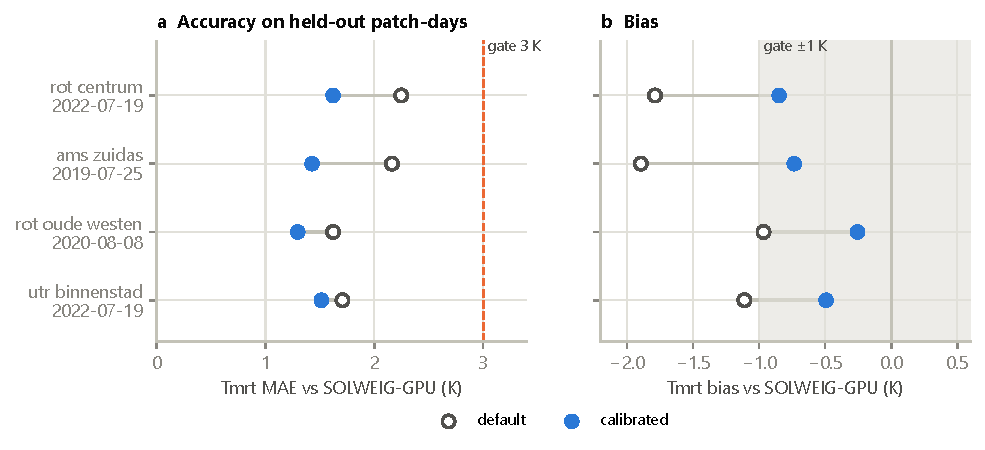
\includegraphics[width=\linewidth]{F1_engine_validation.pdf}
  \caption{Acceptance of the 2.5D engine against SOLWEIG-GPU on four held-out patch-days that were not used for calibration. (a) Mean absolute error and (b) bias of mean radiant temperature over all ground pixel-hours of the 500~m core. Open circles show default parameters and filled circles the parameters calibrated on Amsterdam Grachtengordel, 25 July 2019. The dashed line in (a) marks the 3~K error criterion, and the shaded band in (b) marks the $\pm$1~K bias criterion.}
  \label{fig:F1}
\end{figure}

\begin{table}[tbp]
\centering
\small
\setlength{\tabcolsep}{5pt}
\caption{Mean radiant temperature of the 2.5D engine against SOLWEIG-GPU over all ground pixel-hours of the 500~m core, with default and calibrated parameters. The first row is the calibration patch-day (fit); the others are held out. Acceptance gate: MAE $\le$ 3~K and $|\mathrm{bias}|$ $\le$ 1~K.}
\label{tab:T2_engine_vs_solweig}
\begin{tabular}{lrrrrl}
\toprule
 & \multicolumn{2}{c}{Default} & \multicolumn{2}{c}{Calibrated} & \\
\cmidrule(lr){2-3}\cmidrule(lr){4-5}
Patch and day & MAE (K) & Bias (K) & MAE (K) & Bias (K) & Gate \\
\midrule
Amsterdam Grachtengordel, 25 Jul 2019 & 1.81 & $-$1.36 & 1.32 & $-$0.40 & fit \\
Utrecht Binnenstad, 19 Jul 2022 & 1.71 & $-$1.11 & 1.51 & $-$0.49 & pass \\
Rotterdam Oude Westen, 8 Aug 2020 & 1.62 & $-$0.97 & 1.30 & $-$0.26 & pass \\
Amsterdam Zuidas, 25 Jul 2019 & 2.16 & $-$1.90 & 1.43 & $-$0.73 & pass \\
Rotterdam Centrum, 19 Jul 2022 & 2.25 & $-$1.79 & 1.62 & $-$0.85 & pass \\
\bottomrule
\end{tabular}
\end{table}


\subsection{Physics-informed edges carry generalisation to unseen cities}\label{sec:res-surrogate}

Table~\ref{tab:T3_surrogates} and Fig.~\ref{fig:F2} show the ablation. The sum-aggregation GNN with geometric edges was first selected on held-out plantings of its own training patches. It appeared highly accurate in validation, with a change error of 0.034~\degC, but reached 0.099~\degC{} in Rotterdam and 0.117~\degC{} in Freiburg. With leave-patch-out validation the same model scored 0.100~\degC{} in validation and 0.101~\degC{} in Rotterdam. Most of the apparent gap between seen and unseen patches was thus an artefact of the validation protocol. Dropout and weight decay alone did not improve performance in unseen cities.

Adding the crown-shadow edge features reduced the change error to 0.063~\degC{} in Rotterdam, with a correlation of 0.906 and a UTCI error of 0.062~\degC. In Freiburg the change error was 0.075~\degC, with a correlation of 0.879 and a UTCI error of 0.074~\degC. These errors are 66\% and 61\% below the no-change reference, against 47\% and 39\% with geometric edges only. Validation and unseen-city errors agreed (0.064 versus 0.063~\degC), so no residual gap between seen and unseen patches remained (Fig.~\ref{fig:F3}). On their own, without any model, the summed crown-shadow features correlated at $-0.87$ (Rotterdam Centrum) and $-0.92$ (Amsterdam Bijlmer) with the engine's change in UTCI.

GATv2 attention was worse than predicting no change in both unseen cities. Its errors were 0.291 and 0.277~\degC, with correlations of 0.164 and 0.167. This is consistent with softmax averaging over planted slots, which discards the number of crowns. The 90\% split-conformal half-width, averaged over hours, was $\pm$0.077~\degC{} for the GNN and $\pm$0.082~\degC{} for the linear model. It ranged from 0.04~\degC{} in the early morning to 0.30~\degC{} at the hours of strongest shading. On all counterfactual plantings of the test patches, the GNN's hourly margins covered 90\% of segment-hours when pooled and 86--92\% per patch, close to the nominal 90\%. On the layouts that the optimiser returned, coverage was lower, at 79--89\% per patch and as low as 72\% at single hours. Optimised layouts are not exchangeable with the calibration set, because the optimiser seeks layouts that the surrogate rates favourably, so the nominal guarantee does not carry over to them. This is why every reported outcome was re-simulated with the engine.

\begin{table}[tbp]
\centering
\small
\setlength{\tabcolsep}{5pt}
\caption{Surrogate accuracy on the tree-induced change in segment UTCI in unseen cities. Sum, sum-aggregation GNN; GATv2, attention GNN; v1/v2, edge features without/with crown-shadow and under-crown terms; val., model-selection protocol. MAE, mean absolute error of the change against the engine; $r$, Pearson correlation; skill $= 1 - \mathrm{MAE}/\mathrm{MAE}_0$, where $\mathrm{MAE}_0$ is the error of predicting no change. Rotterdam is an unseen city; Freiburg is an unseen city with imputed building heights.}
\label{tab:T3_surrogates}
\begin{tabular}{lrrrrrr}
\toprule
 & \multicolumn{3}{c}{Rotterdam} & \multicolumn{3}{c}{Freiburg} \\
\cmidrule(lr){2-4}\cmidrule(lr){5-7}
Model & MAE ($^\circ$C) & $r$ & Skill (\%) & MAE ($^\circ$C) & $r$ & Skill (\%) \\
\midrule
GATv2, v1 & 0.291 & 0.164 & $-$57 & 0.277 & 0.167 & $-$44 \\
Sum, v1, within-patch val. & 0.099 & 0.837 & 47 & 0.117 & 0.788 & 39 \\
Sum, v1, leave-patch-out val. & 0.101 & 0.833 & 45 & 0.118 & 0.789 & 39 \\
Linear model, v2 & 0.067 & 0.902 & 64 & 0.089 & 0.865 & 53 \\
Sum, v2 (ours) & 0.063 & 0.906 & 66 & 0.075 & 0.879 & 61 \\
\bottomrule
\end{tabular}
\end{table}


\begin{figure}[t]
  \centering
  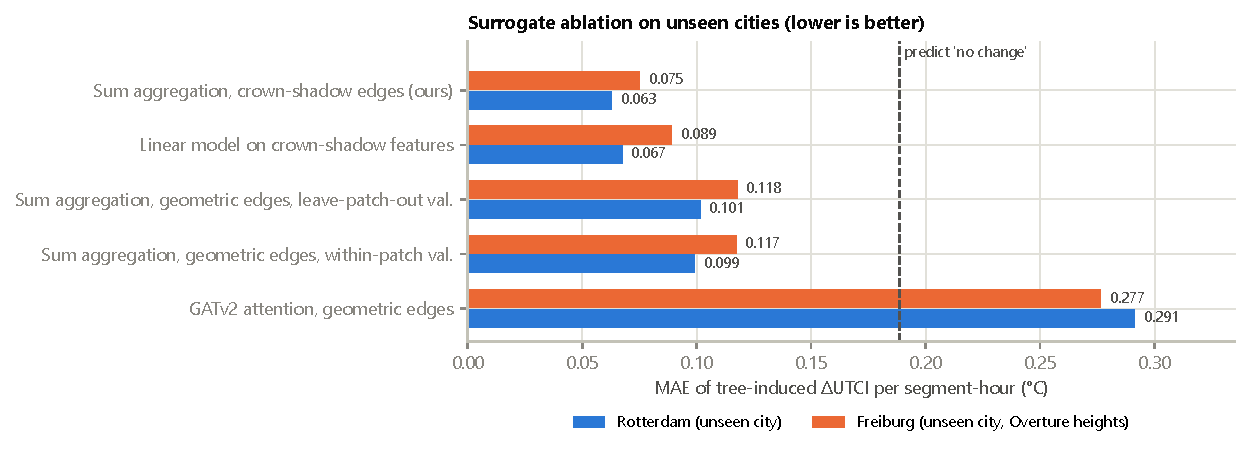
\includegraphics[width=\linewidth]{F2_surrogate_ablation.pdf}
  \caption{Surrogate ablation in unseen cities. Bars give the mean absolute error, relative to the engine, of the tree-induced change in segment UTCI per segment-hour. Rotterdam comprises three patches of an unseen city; Freiburg is an unseen city in another country, with 65.8\% of building heights imputed. The dashed line is the error of predicting that trees change nothing. Models differ in aggregation (sum versus GATv2 attention), in edge features (geometric only versus with crown-shadow and under-crown features) and in validation protocol (held-out plantings versus whole held-out patches). The linear model uses the crown-shadow features without a graph network. Lower is better.}
  \label{fig:F2}
\end{figure}

\begin{figure}[t]
  \centering
  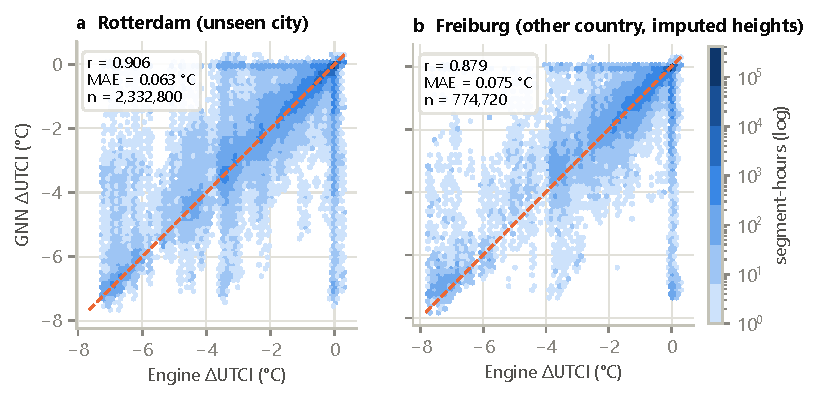
\includegraphics[width=0.9\linewidth]{F3_parity_unseen_cities.pdf}
  \caption{Tree-induced change in segment UTCI predicted by the GNN with crown-shadow edges against the calibrated engine. Panels show every non-baseline planting and hour in (a) the three Rotterdam patches and (b) Freiburg, neither of which was used for training or model selection. Colour gives the number of segment-hours per hexagon on a logarithmic scale, and the dashed line is the 1:1 line. Inset statistics are the Pearson correlation, the mean absolute error and the number of segment-hours.}
  \label{fig:F3}
\end{figure}

\subsection{Where the GNN adds value over a linear model}\label{sec:res-density}

A per-hour linear model on the same physics features came close to the GNN (Table~\ref{tab:T3_surrogates}). Its change error was 0.067~\degC{} in Rotterdam (correlation 0.902) and 0.089~\degC{} in Freiburg (correlation 0.865). The GNN was therefore 7\% more accurate in Rotterdam and 16\% more accurate in Freiburg. Stratifying the unseen-city plantings by planting density locates the difference (Fig.~\ref{fig:F4}). Below 10\% of slots planted, the two models are indistinguishable ($-1$\%). Above that, the GNN's advantage grows to 7\%, 10\% and 11\% in the 10--20\%, 20--30\% and 30--40\% bins, where overlapping crowns break additivity.

\begin{figure}[t]
  \centering
  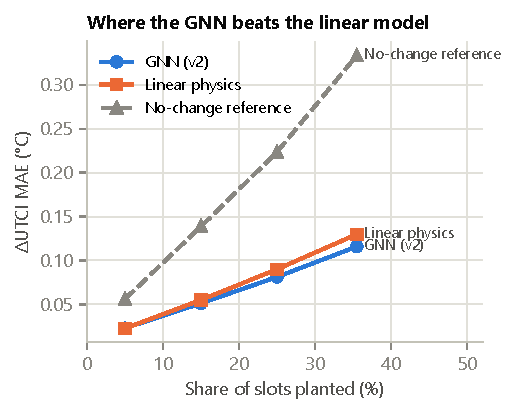
\includegraphics[width=0.55\linewidth]{F4_error_by_density.pdf}
  \caption{Mean absolute error of the tree-induced change in segment UTCI as a function of the share of planting slots planted. Plantings are pooled over the unseen-city patches (Rotterdam and Freiburg). Lines show the GNN with crown-shadow edges, the linear physics model and the no-change reference. Points are the centres of the 0--10\%, 10--20\%, 20--30\% and 30--40\% bins.}
  \label{fig:F4}
\end{figure}

\subsection{Optimised allocation and the strength of greedy}\label{sec:res-bench}

Optimised layouts consistently outperformed random ones in engine-verified heat-dose reduction (Table~\ref{tab:T4_benchmark}, Fig.~\ref{fig:F5}). Across the four test patches and five budgets, the ratio of optimised to random reduction ranged from 1.8 to 6.0. The ratio was largest at low budgets, where choosing the right streets matters most. At 40\% of slots, optimised layouts reduced dose by 4.75--7.25\%, against 2.37--3.75\% for random layouts. Put differently, a quarter to a half as many well-placed trees matched the dose reduction of the largest random planting (Table~\ref{tab:T4_benchmark}).

The practitioner heuristics fell clearly short of model-based allocation. Planting the sunniest, busiest streets achieved 46--85\% of greedy's reduction across patches and budgets, and 1.4--3.3 times the reduction of random layouts. Without the flow weighting, the sun-only rule achieved 29--71\% of greedy's reduction. Both the shading physics and the pedestrian weighting therefore mattered. Sunny streets are not necessarily those where a tree casts useful shade on the walking path at the hours of heat stress, and they are not necessarily the streets that people use.

NSGA-III did not outperform greedy on cooling. Across all patches and budgets, its layouts lay within $-0.05$ to $+0.02$ percentage points of greedy. This held even with 15,001 GNN evaluations and 50,051 linear evaluations per patch, and the two NSGA-III variants and greedy selected essentially the same cooling-optimal layouts. Part of this agreement is built in, because the NSGA-III population was seeded with the greedy layouts. Without that seeding, the same search reached only 60--91\% of greedy's reduction at each budget, and the hypervolume of its front was 2--6\% lower. Greedy is thus hard to beat on cooling, not merely matched by construction. The close performance of the linear surrogate indicates that shading was nearly additive, which makes the dose objective close to a coverage problem. For monotone submodular objectives of this kind, greedy selection is near-optimal~\citep{nemhauser1978}; our dose objective is only approximately of this kind, because of the heat-stress threshold and overlapping crowns.

\begin{table}[tbp]
\centering
\small
\setlength{\tabcolsep}{5pt}
\caption{Engine-verified reduction (\%) of person-weighted heat dose (UTCI $>$ 26~$^\circ$C) by method and tree budget in the four test patches (Freiburg Altstadt is the transfer patch). Random layouts: mean $\pm$ standard deviation of ten layouts.}
\label{tab:T4_benchmark}
\begin{tabular}{lrrrrr}
\toprule
 & & \multicolumn{2}{c}{NSGA-III} & & \\
\cmidrule(lr){3-4}
Patch & Trees (share of slots) & GNN & Linear & Greedy & Random \\
\midrule
Rotterdam Centrum & 12 (5\%) & 1.16 & 1.16 & 1.16 & 0.24 $\pm$ 0.06 \\
 & 25 (10\%) & 2.16 & 2.16 & 2.16 & 0.68 $\pm$ 0.07 \\
 & 50 (20\%) & 3.41 & 3.41 & 3.41 & 1.23 $\pm$ 0.10 \\
 & 75 (30\%) & 4.18 & 4.19 & 4.19 & 1.69 $\pm$ 0.14 \\
 & 100 (40\%) & 4.75 & 4.75 & 4.75 & 2.37 $\pm$ 0.20 \\
\addlinespace
Rotterdam Kop van Zuid & 12 (5\%) & 1.34 & 1.34 & 1.34 & 0.38 $\pm$ 0.09 \\
 & 25 (10\%) & 2.25 & 2.25 & 2.25 & 0.65 $\pm$ 0.08 \\
 & 50 (20\%) & 3.57 & 3.57 & 3.57 & 1.52 $\pm$ 0.12 \\
 & 75 (30\%) & 4.63 & 4.63 & 4.63 & 2.14 $\pm$ 0.19 \\
 & 100 (40\%) & 5.52 & 5.52 & 5.52 & 2.99 $\pm$ 0.28 \\
\addlinespace
Rotterdam Oude Westen & 12 (5\%) & 2.35 & 2.35 & 2.35 & 0.39 $\pm$ 0.11 \\
 & 25 (10\%) & 3.89 & 3.89 & 3.89 & 0.91 $\pm$ 0.20 \\
 & 50 (20\%) & 5.64 & 5.65 & 5.65 & 1.74 $\pm$ 0.14 \\
 & 75 (30\%) & 6.54 & 6.54 & 6.54 & 2.80 $\pm$ 0.36 \\
 & 100 (40\%) & 7.25 & 7.25 & 7.25 & 3.75 $\pm$ 0.37 \\
\addlinespace
Freiburg Altstadt & 12 (5\%) & 1.21 & 1.21 & 1.21 & 0.39 $\pm$ 0.11 \\
 & 25 (10\%) & 2.28 & 2.26 & 2.26 & 0.81 $\pm$ 0.11 \\
 & 50 (20\%) & 3.75 & 3.80 & 3.80 & 1.56 $\pm$ 0.14 \\
 & 75 (30\%) & 4.91 & 4.91 & 4.91 & 2.47 $\pm$ 0.22 \\
 & 100 (40\%) & 5.77 & 5.77 & 5.77 & 3.25 $\pm$ 0.26 \\
\bottomrule
\end{tabular}
\end{table}


\begin{figure}[t]
  \centering
  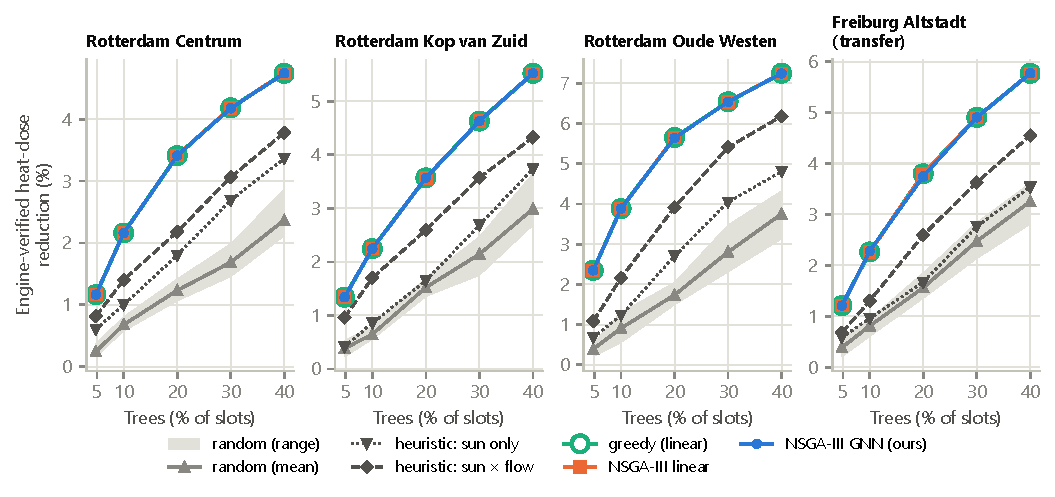
\includegraphics[width=\linewidth]{F5_benchmark_unseen_cities.pdf}
  \caption{Engine-verified reduction of person-weighted heat dose in the four test patches as a function of the number of trees. Dose counts UTCI above 26~\degC, weighted by gravity-model pedestrian flow and time on segment. The number of trees is expressed as a share of the 250 candidate slots. Greedy allocation (open circles), NSGA-III on the linear surrogate (squares) and NSGA-III on the GNN (small filled circles) largely coincide. Dashed and dotted grey lines are the practitioner heuristics with and without flow weighting. Random layouts are shown as the mean (triangles) and range (band) of ten layouts per budget.}
  \label{fig:F5}
\end{figure}

\subsection{Equity trade-offs available on the Pareto front}\label{sec:res-equity}

The value of the multi-objective search lies in trade-offs that greedy cannot represent. At every budget we searched the NSGA-III (GNN) front among layouts keeping at least 90\% of greedy's engine-verified cooling. Among these we selected the layout with the lowest between-district Theil index (Table~\ref{tab:T5_equity}). Such layouts reduced the Theil index by up to 8.2\% (Rotterdam Oude Westen, 75 trees). In the other patches they reduced it by 2.8--5.1\% at budgets of 50--100 trees, while retaining 90--100\% of greedy's cooling. Gains at the lowest budgets were small (0.0--1.7\%).

The per-district dose reductions show how these gains arise. In 19 of the 20 patch--budget combinations, the equity-selected layout gave the district with the lowest per-capita dose less cooling than greedy did, by up to 2.79 percentage points. The district with the highest per-capita dose received more cooling in 15 combinations, but by at most 1.61 percentage points and with a median of 0.15. The lower Theil index therefore came mainly from cooling the least exposed district less, not from cooling the most exposed district more. No district received more dose than without new trees, so the equity layouts do not level down in absolute terms. They redistribute a slightly smaller cooling benefit towards a more even outcome. The districts are ranked here by modelled dose per unit of floor area, not by social deprivation.

Repeating the NSGA-III run with five random seeds showed that the cooling results are stable but the equity results are not. The dose reduction of the layout picked at each budget varied between seeds by a standard deviation of at most 0.02 percentage points and stayed within $-0.05$ to $+0.03$ points of greedy. For equity we searched a subsample of 100 front layouts per seed. A layout that kept 90\% of greedy's cooling and lowered the Theil index was found in 68 of the 100 patch--budget--seed combinations, with a median change of $-2.7$\%. At a given patch and budget, the change varied between seeds by a standard deviation of up to 6.3 percentage points, and in 3 combinations the best available layout was less equal than greedy. The equity trade-offs in Table~\ref{tab:T5_equity} should therefore be read as examples of what a multi-objective search can find, with the 8.2\% reduction as a favourable case, rather than as stable estimates.

Fig.~\ref{fig:F6} shows the front for Rotterdam Centrum. At a given number of trees, layouts with slightly lower cooling achieve lower Theil values. The map shows where the knee layout places its trees and the cooling that SOLWEIG-GPU simulates for it.

\begin{table}[tbp]
\centering
\small
\caption{Between-district equity available on the NSGA-III (GNN) front at $\ge$ 90\% of greedy's engine-verified cooling. Theil index of per-capita dose across four districts, with building floor area as population proxy (lower is more equal).}
\label{tab:T5_equity}
\begin{tabular}{lrrrrr}
\toprule
 & & \multicolumn{2}{c}{Theil index} & & \\
\cmidrule(lr){3-4}
Patch & Trees & Greedy & Best front & Change (\%) & Cooling kept (\%) \\
\midrule
Rotterdam Centrum & 12 & 0.0681 & 0.0669 & $-$1.7 & 92 \\
 & 25 & 0.0673 & 0.0666 & $-$1.0 & 93 \\
 & 50 & 0.0671 & 0.0652 & $-$2.8 & 90 \\
 & 75 & 0.0666 & 0.0645 & $-$3.1 & 90 \\
 & 100 & 0.0667 & 0.0641 & $-$3.9 & 90 \\
\addlinespace
Rotterdam Kop van Zuid & 12 & 0.1094 & 0.1084 & $-$0.9 & 93 \\
 & 25 & 0.1078 & 0.1078 & 0.0 & 100 \\
 & 50 & 0.1050 & 0.1014 & $-$3.4 & 92 \\
 & 75 & 0.1040 & 0.0988 & $-$5.0 & 90 \\
 & 100 & 0.1032 & 0.1004 & $-$2.8 & 93 \\
\addlinespace
Rotterdam Oude Westen & 12 & 0.0361 & 0.0356 & $-$1.6 & 91 \\
 & 25 & 0.0346 & 0.0341 & $-$1.6 & 95 \\
 & 50 & 0.0346 & 0.0333 & $-$3.6 & 92 \\
 & 75 & 0.0338 & 0.0311 & $-$8.2 & 93 \\
 & 100 & 0.0326 & 0.0316 & $-$3.3 & 91 \\
\addlinespace
Freiburg Altstadt & 12 & 0.0820 & 0.0813 & $-$0.9 & 97 \\
 & 25 & 0.0813 & 0.0804 & $-$1.2 & 92 \\
 & 50 & 0.0817 & 0.0794 & $-$2.9 & 94 \\
 & 75 & 0.0819 & 0.0778 & $-$5.1 & 93 \\
 & 100 & 0.0817 & 0.0781 & $-$4.4 & 92 \\
\bottomrule
\end{tabular}
\end{table}


\begin{figure}[t]
  \centering
  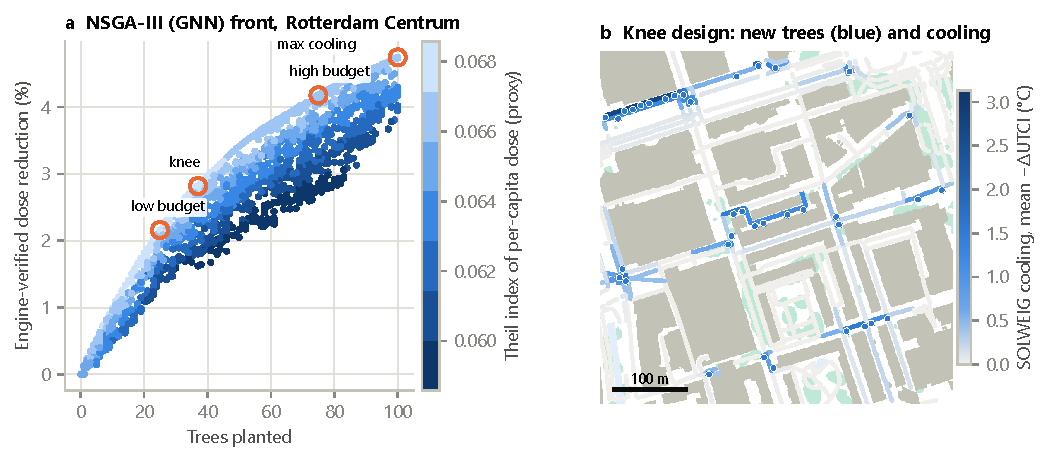
\includegraphics[width=\linewidth]{F6_pareto_front_and_map.pdf}
  \caption{Pareto front and knee layout for Rotterdam Centrum, an unseen city. (a) NSGA-III (GNN) front of engine-verified dose reduction against the number of trees. Colour gives the engine-verified Theil index of per-capita dose across four districts, with building floor area as population proxy; darker is more equal. Orange circles mark the five layouts verified with SOLWEIG-GPU. (b) Map of the knee layout. Buildings are grey, existing canopy green and water light blue; new trees are blue points. Street segments are coloured by the mean cooling simulated by SOLWEIG-GPU over 08:00--19:00 on the three heatwave days. The scale bar is 100~m.}
  \label{fig:F6}
\end{figure}

\subsection{Sensitivity to modelling choices}\label{sec:res-sens}

Table~\ref{tab:T7_sensitivity} summarises the sensitivity analysis. The size of the new trees mattered most for the magnitude of cooling. With young crowns the greedy layouts reduced dose at 40\% of slots by 2.30--3.39\%, and with mature crowns by 7.77--11.55\%, against 4.75--7.25\% with the reference crown. Crown transmissivity, the street wind factor, the gravity decay and the heat-stress threshold changed this reduction much less. The comparisons between methods held in every setting. Greedy layouts reduced dose at least 1.7 times more than random layouts, and the sun $\times$ flow heuristic never exceeded 88\% of greedy's reduction. When the objective changed, the re-optimised greedy layouts overlapped strongly with the reference layouts, with a Jaccard index of 0.71--1.00, and re-optimising gained at most 0.06 percentage points of dose reduction. The choice of streets is therefore robust to the uncertain flow and threshold parameters. The main uncertainty in the size of the benefit is how large the planted trees grow.

\begin{table}[tbp]
\centering
\footnotesize
\setlength{\tabcolsep}{4pt}
\caption{Sensitivity of the allocation results to fixed modelling choices, as ranges over the four test patches and five budgets (engine-verified). Physical settings re-simulate the layouts optimised under the reference setting; objective settings re-run greedy under the new objective, and the overlap is the Jaccard index of its planted slots with the reference greedy layout. Greedy reduction is at 40\% of slots. Gravity decay is $\beta$ of the pedestrian-flow model.}
\label{tab:T7_sensitivity}
\begin{tabular}{lrrrr}
\toprule
Setting & \makecell[r]{Greedy reduction\\at 40\% (\%)} & \makecell[r]{Greedy /\\random} & \makecell[r]{Heuristic share\\of greedy (\%)} & \makecell[r]{Slot overlap\\with reference} \\
\midrule
Reference setting & 4.75–7.25 & 1.8–6.0 & 46–85 & -- \\
Crown transmissivity 0.01 & 4.85–7.43 & 1.8–6.0 & 46–85 & -- \\
Crown transmissivity 0.10 & 4.36–6.62 & 1.8–6.0 & 46–85 & -- \\
Young crown (2 m radius, 6 m) & 2.30–3.39 & 1.9–7.7 & 46–81 & -- \\
Mature crown (4 m radius, 12 m) & 7.77–11.55 & 1.7–4.6 & 57–88 & -- \\
Street wind factor 0.3 & 4.70–7.17 & 1.8–6.0 & 46–85 & -- \\
Street wind factor 0.7 & 4.84–7.42 & 1.8–6.0 & 46–85 & -- \\
Gravity decay 0.001 per m & 4.77–7.27 & 1.8–5.8 & 46–85 & 0.85–1.00 \\
Gravity decay 0.004 per m & 4.69–7.22 & 1.8–6.4 & 46–86 & 0.71–0.96 \\
UTCI threshold 24 $^\circ$C & 4.07–6.22 & 1.8–6.0 & 47–85 & 0.85–1.00 \\
UTCI threshold 28 $^\circ$C & 5.60–8.52 & 1.8–5.8 & 46–86 & 0.71–1.00 \\
\bottomrule
\end{tabular}
\end{table}


\subsection{Cross-model verification with SOLWEIG-GPU}\label{sec:res-verify}

SOLWEIG-GPU confirmed the cooling of all four optimised layouts in Rotterdam Centrum (Table~\ref{tab:T6_solweig_verification}, Fig.~\ref{fig:F7}). It reduced heat dose by 2.40, 3.20, 5.08 and 5.92\% for the low-budget, knee, high-budget and maximum-cooling layouts. Our engine gave 2.16, 2.82, 4.18 and 4.75\%, and the GNN 2.14, 2.79, 4.09 and 4.66\%. Our chain was therefore conservative. It underestimated the SOLWEIG reduction by 10--20\% (engine) and 11--21\% (GNN).

At the level of individual segment-hours, the change in UTCI correlated with SOLWEIG at 0.95--0.97 for the engine and 0.91--0.94 for the GNN. The models differed in where the cooling fell, not only in how much. We compared them on a common mask, the segment-hours that SOLWEIG cooled by more than 0.05~\degC{} (Table~\ref{tab:T6_solweig_verification}). On this mask the engine's mean cooling was 6--16\% smaller than SOLWEIG's. Where SOLWEIG cooled by more than 1~\degC, beneath and beside the new crowns, the engine cooled more, by 0.12--0.39~\degC{} on average. Elsewhere on the mask it cooled less, by 0.12--0.20~\degC. The engine also cooled only 32--36\% as many segment-hours as SOLWEIG did. SOLWEIG's cooling was therefore spatially broader and less peaked. Its strongest segment cooling was $-6.07$~\degC, against $-7.25$~\degC{} for the engine. This is consistent with the shaded-stratum bias of Section~\ref{sec:res-engine}, since our engine lacks SOLWEIG's anisotropic sky and per-aspect wall long-wave fluxes.

\begin{table}[tbp]
\centering
\small
\setlength{\tabcolsep}{4.5pt}
\caption{Independent SOLWEIG-GPU verification of five Pareto designs in Rotterdam Centrum, an unseen city. Dose reduction is relative to each model's own run without new trees; $\Delta$UTCI is the mean over affected segment-hours; $r$ is the per-segment-hour correlation of $\Delta$UTCI between the GNN and SOLWEIG-GPU.}
\label{tab:T6_solweig_verification}
\begin{tabular}{lrrrrrrrr}
\toprule
 & & \multicolumn{3}{c}{Dose reduction (\%)} & \multicolumn{3}{c}{Mean $\Delta$UTCI ($^\circ$C)} & \\
\cmidrule(lr){3-5}\cmidrule(lr){6-8}
Design & Trees & SOLWEIG & Engine & GNN & SOLWEIG & Engine & GNN & $r$ \\
\midrule
None & 0 & 0.00 & 0.00 & 0.00 & 0.00 & 0.00 & 0.00 & -- \\
Low budget & 25 & 2.40 & 2.16 & 2.14 & $-$0.63 & $-$1.88 & $-$1.68 & 0.94 \\
Knee & 37 & 3.20 & 2.82 & 2.79 & $-$0.70 & $-$1.90 & $-$1.73 & 0.94 \\
High budget & 75 & 5.08 & 4.18 & 4.09 & $-$0.77 & $-$1.91 & $-$1.74 & 0.91 \\
Max cooling & 100 & 5.92 & 4.75 & 4.66 & $-$0.80 & $-$1.86 & $-$1.72 & 0.91 \\
\bottomrule
\end{tabular}
\end{table}


\begin{figure}[t]
  \centering
  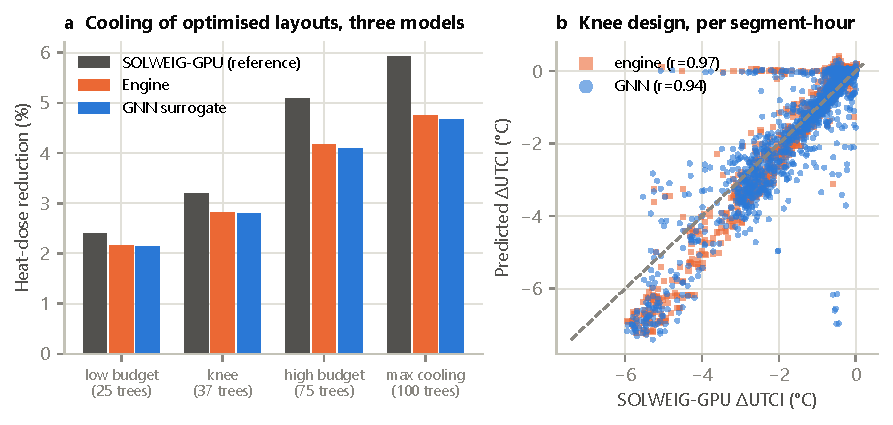
\includegraphics[width=\linewidth]{F7_solweig_verification.pdf}
  \caption{Cross-model verification of optimised layouts in Rotterdam Centrum with SOLWEIG-GPU. (a) Reduction of person-weighted heat dose for four layouts from the NSGA-III (GNN) front. Bars compare SOLWEIG-GPU (reference), the calibrated engine and the GNN, each relative to its own run without new trees. (b) Change in segment UTCI for the knee layout per segment-hour over 08:00--19:00 on the three heatwave days. The engine (squares) and the GNN (circles) are plotted against SOLWEIG-GPU. The dashed line is the 1:1 line, and the legend gives Pearson correlations.}
  \label{fig:F7}
\end{figure}

%% ==========================================================================================
\section{Discussion}\label{sec:discussion}

\subsection{Mechanism-level features, not model capacity, carry transfer}

Generalisation to an unseen city and to another country's input regime came from describing the shading mechanism on the graph edges, not from a more expressive network. A linear model on the crown-shadow features came within 7\% of the GNN in Rotterdam. The GNN's remaining advantage grew with planting density and under the input shift in Freiburg. These are the conditions in which overlapping crowns and imputed geometry interact. Our design shares the aim of recent physics-informed graph models for urban microclimate~\citep{xin2025}, but here the physics enters through intervention-specific edges.

Two further lessons apply to surrogate-assisted planning beyond trees. First, validating on held-out \emph{interventions} of training scenes overstates transfer, so whole held-out scenes are needed. Second, the aggregation operator must respect how interventions combine. Attention normalises away the number of trees, which made GATv2 worse than predicting no change.

\subsection{What multi-objective optimisation adds}

NSGA-III did not improve cooling over greedy allocation, even with 15,001 GNN evaluations per patch, and without greedy seeding it fell short of greedy. When interventions act nearly additively, greedy is a strong, transparent and cheap baseline~\citep{nemhauser1978}. We suggest that studies proposing multi-objective or learned optimisers for tree placement report it, together with an unseeded run of their optimiser.

\subsection{Implications for tree-planting practice}

For planners, most of the benefit comes from \emph{which} streets receive trees. Optimised placement achieved 1.8--6.0 times the reduction of random placement, and a quarter to a half as many well-placed trees matched the largest random planting. Common rules of thumb capture only part of this benefit. Planting the sunniest, busiest streets achieved 46--85\% of the model-based reduction, and ignoring pedestrian flow lowered this to 29--71\%. The gap arises because the cooling a tree gives depends on where its shadow falls during the hours of heat stress, relative to the walking path and to the shade that buildings already cast.

The decision-relevant model is nevertheless simple. A linear model on the crown-shadow features combined with greedy allocation reached the cooling optimum. A municipality can therefore rank candidate positions with a transparent shading calculation and a pedestrian-flow estimate, and use a fuller surrogate where planting is dense or where equity trade-offs are needed. Our method assumes that every candidate slot is plantable. In practice, below-ground utilities, sidewalk width, sight lines and species choice remove many positions. The ranking can be applied to the plantable subset after these constraints are mapped, but we did not test how much the constraints change the attainable cooling. The benefit also depends strongly on how large the trees grow. Young crowns gave about half and mature crowns about one and a half times the dose reduction of the reference crown (Section~\ref{sec:res-sens}). The cooling estimated here should therefore be read as a benefit that builds up over years of growth, which favours species and planting conditions that let crowns reach full size.

The multi-objective front adds what greedy cannot provide: explicit trade-offs between total cooling, distributional equity and budget. At 90\% of greedy's cooling, the between-district Theil index fell by up to 8.2\%. These gains are modest because new trees remove only a few percent of total dose. They therefore cannot reverse inequality that is driven by the unplanted street environment. The per-district results also show what the more equal layouts do. They mostly withhold cooling from the least exposed district rather than add cooling where dose is highest. A planner who wants to target the most exposed district should therefore constrain the allocation directly, for example with a minimum share of trees per district, instead of relying on an inequality index alone. The front makes this trade-off visible and quantifies its cost in total cooling, although the size of the equity gain varied between optimiser runs.

\subsection{Decision reliability}

Two elements support the recommended layouts beyond the surrogate's own predictions:
\begin{itemize}
  \item every reported outcome was re-simulated by the physics engine;
  \item a second model, SOLWEIG-GPU, developed independently of our engine, confirmed the cooling of optimised layouts in an unseen city.
\end{itemize}
The independent model found 10--20\% \emph{more} cooling than the engine, so the reported totals are, if anything, conservative. This holds for totals, not for every street. Directly under the new crowns the engine cooled more than SOLWEIG, by up to 0.39~\degC{} on average, while SOLWEIG spread a weaker cooling over about three times as many segment-hours. A planner should therefore read the predicted cooling of a single planted street as an upper estimate and the predicted total benefit as a lower one. The correlation of 0.91--0.94 between GNN and SOLWEIG changes shows that the surrogate ranks streets consistently with the reference model. Both checks compare models with each other; neither replaces field measurement of \tmrt{} under new trees. The hourly conformal margin does not add a third guarantee. It calibrates the heat-stress threshold for surrogate error on held-out patches, but its coverage on optimised layouts fell below the nominal level (Section~\ref{sec:res-surrogate}). Re-simulation, not the margin, therefore underpins the reported outcomes.

\subsection{Limitations}\label{sec:limitations}

\paragraph{Population proxy.} District population, which weights the equity objective, was approximated by building floor area derived from 3DBAG heights, and all vulnerability weights were set to one. Floor area includes offices, retail and other non-residential space. It therefore represents the people present in buildings rather than residents, and it ignores age structure and other drivers of heat vulnerability. The dose itself accrues to pedestrians on a district's streets, who are not necessarily its residents or workers. The four districts are geometric quadrants of the core, so the Theil index also depends on where the quadrant boundaries fall. The equity results (Table~\ref{tab:T5_equity}) demonstrate the method and the size of the trade-off under this proxy. They are not estimates of distributional effects on residents. Census population and age structure must replace the proxy before equity conclusions are drawn for specific neighbourhoods.

\paragraph{Uniform trip generation.} The gravity model generated the same number of trips at every network node and used Overture places as destinations. It was not calibrated against pedestrian counts, and it uses shortest paths and one flow pattern for all hours. Flow weights determine which streets the dose objective favours. Other trip-generation assumptions, such as residential origins or transit-weighted destinations, could therefore change the selected layouts. They would not change the physics of tree cooling.

\paragraph{Single-patch, model-only verification.} The SOLWEIG-GPU verification covers four optimised layouts in one patch, Rotterdam Centrum, on three heatwave days. Its spatial agreement and conservative bias are encouraging, but they are not established for other morphologies. In particular, the shaded-stratum bias in high-rise districts (Section~\ref{sec:res-engine}) suggests that agreement may be weaker there. Verification on further patches, including Freiburg, would strengthen the claim. Both the engine acceptance gate and the layout verification use SOLWEIG-GPU as the reference, so neither tests absolute \tmrt{} against observations. Field measurements under newly planted trees are needed to confirm the absolute size of the cooling.

\paragraph{Further limitations.} The engine is 2.5D and radiative. It does not model wind fields, crown evapotranspiration or the effect of trees on air temperature. It also simplifies wall and ground temperatures and sky anisotropy relative to SOLWEIG, and its calibration used a single fitting patch-day. New trees had one crown geometry (3~m radius, 8~m height) with leaf-on transmissivity. The analysis covers 36 daytime hours on three heatwave days rather than a season. The canopy map has a reported error of 2.8~m~\citep{tolan2024}, and 65.8\% of Freiburg's building heights were imputed. Conformal coverage holds marginally for exchangeable data. Layouts selected by the optimiser are not exchangeable with the calibration set, so their coverage is checked by re-simulation rather than guaranteed. All results use one trained GNN; the stability check covers the optimiser's random seed but not the surrogate's training seed. Finally, apart from Freiburg, all patches lie in the temperate maritime climate of the Netherlands.

%% ==========================================================================================
\section{Conclusions}\label{sec:conclusions}

Where street trees go matters as much as how many are planted. Exposure-weighted allocation, verified by physics simulation in four unseen neighbourhoods, reduced pedestrian heat dose 1.8--6.0 times more than random layouts. A practitioner rule that plants the sunniest, busiest streets captured only 46--85\% of that benefit. Most of the attainable cooling came from a transparent combination of physics-informed shading features, pedestrian flows and greedy allocation. Multi-objective search did not add cooling, but it made the trade-off between cooling and between-district equity explicit. A GNN surrogate with physics-informed crown-shadow edges predicted tree-induced UTCI change in an unseen city with an error of 0.063~\degC{} and a correlation of 0.906. In a German city with largely imputed building heights its error was 0.075~\degC. A cross-model check with SOLWEIG-GPU confirmed the cooling of optimised layouts. Our chain underestimated their total cooling but concentrated it more tightly under the new crowns. Future work should replace the population proxy with census data and calibrate pedestrian flows against counts. It should also extend SOLWEIG verification to more morphologies, test the cooling against field measurements, restrict candidate positions to plantable ones and add tree effects on air temperature and seasonal crown dynamics.

%% ==========================================================================================
\section*{CRediT authorship contribution statement}
\noindent\textbf{Mohammad Baradaran Aghghaleh:} Conceptualization, Methodology, Software, Validation, Formal analysis, Data curation, Writing -- original draft, Visualization.\par
\noindent\textbf{Khorshid Mehrabi:} Conceptualization, Investigation, Validation, Writing -- review \& editing.\par
\noindent\textbf{Ali Yazdani:} Conceptualization, Methodology, Supervision, Writing -- review \& editing.

\section*{Declaration of competing interest}
The authors declare that they have no known competing financial interests or personal relationships that could have appeared to influence the work reported in this paper.

\section*{Funding}
This research did not receive any specific grant from funding agencies in the public, commercial, or not-for-profit sectors.

\section*{Data and code availability}
All input data are open and were accessed on 25 November 2026. 3DBAG and the Open-Meteo archive are distributed under the Creative Commons Attribution 4.0 licence (CC BY 4.0). The walkable network, destinations and water polygons derive from OpenStreetMap through Overture Maps and are \copyright{} OpenStreetMap contributors, available under the Open Database Licence (ODbL). The global 1~m canopy height map is used under its providers' terms. The analysis code, configuration and frozen-dataset hash record are available at \url{https://github.com/mohammadbaradaranaghghaleh/heatgraph-street-trees}. The repository provides a single command, \texttt{reproduce.py}, that regenerates every figure and table from the released results and checks them against the published versions, and an interactive dashboard that shows the layouts and their cooling for every test patch. The released results (processed scenes, counterfactual labels, trained surrogates, and the benchmark and verification outputs, with a checksum for every file) will be deposited in a Zenodo archive with a DOI on publication. Code and data are available to reviewers from the corresponding author on request.

\section*{Declaration of generative AI and AI-assisted technologies in the writing process}
During the preparation of this work the authors used Claude (Anthropic) in order to assist with software development, data analysis scripting, literature organization, and language editing. After using this tool, the authors reviewed, verified, and edited the content and code as needed and take full responsibility for the content of the published article.

\bibliographystyle{elsarticle-harv}
\bibliography{references}

\clearpage
\appendix
\setcounter{table}{0}
\newgeometry{a4paper,margin=1.8cm}
\begin{landscape}
\section{Study patches}\label{app:patches}
\begin{table}[!h]
\centering
\footnotesize
\setlength{\tabcolsep}{3.5pt}
\caption{Study patches: morphology of the 500~m core, source of building heights and role in the experiments. LCZ, Local Climate Zone; BSF, building surface fraction; $h_\mathrm{aw}$, area-weighted building height. Test patches were used only for evaluation; Freiburg is the transfer patch with imputed heights.}
\label{tab:T1_patches}
\begin{tabular}{llllrrrrrrr}
\toprule
 & & & & & & & Towers & Water & Canopy & Walking \\
Patch & Intended LCZ & Role & Heights & Buildings & BSF & $h_\mathrm{aw}$ (m) & $>$40 m & fraction & $>$2 m (\%) & network (km) \\
\midrule
Almere Centrum & LCZ5 planned open midrise & train & 3DBAG & 683 & 0.48 & 14.9 & 0 & 0.02 & 2.5 & 55.4 \\
Amersfoort Vathorst & LCZ6 suburban lowrise & validation & 3DBAG & 2921 & 0.21 & 8.6 & 0 & 0.09 & 5.3 & 42.8 \\
Amsterdam Bijlmer & LCZ4 open highrise & train & 3DBAG & 785 & 0.42 & 14.6 & 0 & 0.05 & 10.4 & 42.5 \\
Amsterdam Bos en Lommer & LCZ2/5 compact-open midrise & validation & 3DBAG & 1488 & 0.28 & 17.4 & 2 & 0.0 & 15.5 & 46.5 \\
Amsterdam Grachtengordel & LCZ2 compact midrise & train & 3DBAG & 2276 & 0.43 & 16.3 & 0 & 0.17 & 9.0 & 35.1 \\
Amsterdam IJburg & LCZ5 open midrise & train & 3DBAG & 1396 & 0.28 & 14.6 & 0 & 0.19 & 0.5 & 39.6 \\
Amsterdam Zuidas & LCZ1/4 highrise & train & 3DBAG & 277 & 0.35 & 45.0 & 19 & 0.01 & 7.3 & 43.1 \\
Den Haag Beatrixkwartier & LCZ1/4 office highrise & train & 3DBAG & 361 & 0.2 & 42.8 & 7 & 0.07 & 24.0 & 50.1 \\
Den Haag Schilderswijk & LCZ2/3 compact low-midrise & train & 3DBAG & 2847 & 0.4 & 10.7 & 0 & 0.02 & 7.5 & 51.7 \\
Delft Campus & LCZ5/9 open campus & train & 3DBAG & 509 & 0.34 & 15.4 & 1 & 0.03 & 18.6 & 43.4 \\
Eindhoven Strijp-S & LCZ8/10 converted industrial & validation & 3DBAG & 1182 & 0.31 & 28.6 & 10 & 0.0 & 8.3 & 59.8 \\
Groningen Binnenstad & LCZ2 compact midrise & train & 3DBAG & 2575 & 0.57 & 14.9 & 2 & 0.0 & 7.0 & 36.1 \\
Rotterdam Centrum & LCZ1/4 highrise & test & 3DBAG & 575 & 0.49 & 32.2 & 17 & 0.01 & 8.0 & 46.0 \\
Rotterdam Kop van Zuid & LCZ4/5 waterfront highrise & test & 3DBAG & 497 & 0.22 & 44.6 & 9 & 0.15 & 4.0 & 39.0 \\
Rotterdam Oude Westen & LCZ2 compact midrise & test & 3DBAG & 2240 & 0.36 & 13.5 & 0 & 0.0 & 23.2 & 35.4 \\
Utrecht Binnenstad & LCZ2/3 historic compact & train & 3DBAG & 2759 & 0.6 & 14.1 & 3 & 0.03 & 12.9 & 42.2 \\
Utrecht Leidsche Rijn & LCZ6 open lowrise & train & 3DBAG & 598 & 0.24 & 20.1 & 0 & 0.01 & 1.6 & 50.9 \\
Freiburg Altstadt & LCZ2 compact midrise & transfer & Overture & 1595 & 0.56 & 16.8 & 2 & 0.0 & 14.3 & 42.8 \\
\bottomrule
\end{tabular}
\end{table}

\end{landscape}
\restoregeometry

\end{document}
